\documentclass[12pt, a4paper]{article}

\usepackage[italian]{babel}
\usepackage[utf8]{inputenc}
\usepackage[T1]{fontenc}
\usepackage{graphicx}
\usepackage{subfig}
\usepackage{caption}
\usepackage{geometry}
\usepackage{color}
\usepackage{amsmath}
\usepackage{amssymb}
\usepackage{booktabs}
\usepackage{tabularx}
\usepackage{wrapfig}
\geometry{a4paper,top=1.5cm,bottom=2cm,left=1.25cm,right=1.5cm,heightrounded,bindingoffset=5mm}
\author{ Marasciulli Andrea \qquad  Lorenzetti Giacomo \qquad Browne Roberto}
\date{\today}
\frenchspacing 
\begin{document}

\begin{section}*{Calibrazione}

Abbiamo variato l'alimentazione dei vari PMT per vedere come cambia il numero di conteggi. I risultati di queste misure sono  riportati nel grafico di \emph{Figura \ref{tensio}}. 

\begin{figure}[h]
\centering
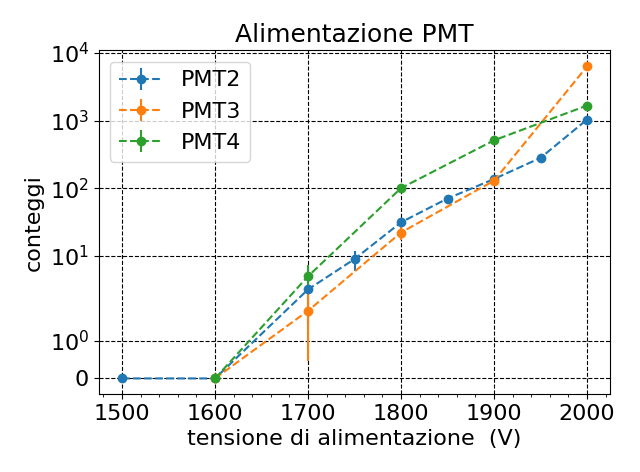
\includegraphics[width=8 cm]{tensio_pmt}
\caption{Numero di conteggi in funzione della tensione di alimentazione}
\label{tensio}
\end{figure}

Il grafico mostra chiaramente l'assenza di qualsiasi $plateau$ tranne nei punti a conteggio nullo. Abbiamo deciso di alimentare i PMT a 1800\! V perché la derivata in quel punto è minore di quella corrispondente a 1900\! V e ci sono abbastanza conteggi da permetterci una loro analisi statistica.

Dal \emph{Particle Physics Booklet 2016} sappiamo che il flusso di raggi cosmici è mediamente 180~Hz$/$\!m$^2$s. Essendo il nostro rivelatore di area $A=l_1l_2=48.0\pm0.1$\! cm $\cdot \, 40.0\pm0.1$\! cm$=1920\pm6$\! cm$^2$ ci aspettiamo il passaggio di 34.6$\pm$0.1 particelle$/$s. Questo numero è simile ai conteggi ottenuti a 1800\! V con soglia V$_{thr}\simeq-376$\! mV. 

\end{section}


\begin{section}*{Modulo di coincidenze}

Per effettuare il conteggio delle coincidenze abbiamo collegato le uscite dei discriminatori al modulo di coincidenze FE260 e la sua uscita al canale 5 dello scaler. I canali 1 e 2 di quest'ultimo sono collegati al PMT4 e al PMT2 attraverso il discriminatore. Le soglie di entrambi sono massime, ovvero $-0.410\pm0.002$\! V misurate dal testpoint. Con questi settaggi i nostri rivelatori misurano circa 40 eventi al secondo, quindi facciamo un calcolo approssimativo del rate di coincidenze casuali usando la formula $R_C=R_1R_2\Delta t$. Siccome il modulo di coincidenze scatta quando c'è una sovrapposizione  di due segnali di livello 1 per più di 1.5\! ns, possiamo dire che il $\Delta t$ vale circa il doppio della durata dell'uscita del discriminatore, ovvero 80\! ns. Abbiamo allora $R_C\simeq 128\cdot10^{-6}\approx1\cdot10^{-4}$, ovvero una coincidenza casuale ogni 3 ore.

\end{section}


\begin{section}*{Tempi di propagazione dei segnali}

Usiamo l'oscilloscopio per visualizzare le coincidenze, ovvero colleghiamo i due discriminatori utilizzati al nostro strumento ed osserviamo degli impulsi NIM quasi simultanei, in particolare vediamo che il segnale che arriva più tardi si discosta solo di qualche nanosecondo da quello precedente, ma questa asincronia non ci causa nessun problema perché vale al massimo il 10\% della lunghezza dei nostri impulsi.
% chiedere a Giacomo se ha già scritto perché abbiamo scelto l'ampiezza massima 
Ciò non dovrebbe mascherare l'arrivo di una seconda coincidenza in quell'intervallo di tempo perché il rate atteso è di decine di hertz, come già detto nella sezione \textbf{calibrazione}, che equivale in media al passaggio di un raggio cosmico ogni decimo di secondo in caso di accettanza geometrica unitaria.

Per trovare il miglior punto di lavoro inseriamo nel crate due \emph{delay unit} che colleghiamo in serie ai discriminatori di cui sopra. Prima di effettuare i conteggi testiamo una delay unit mandandole in ingresso l'onda quadra data dal clock dello scaler. Confermiamo che il ritardo minimo introdotto da questo modulo è 2.5$\pm$0.2\! ns e che tutti gli altri inseribili sono compatibili con quanto dichiarato con un'accuratezza del 10\%. La \emph{Figura \ref{curv}} mostra la curva di cavo che, come atteso, mostra un massimo di conteggi quando il ritardo relativo è inferiore alla durata dell'impulso del discriminatore ed è quasi nulla altrove. La variabile utilizzata è $\Delta t=D2-D4$ dove questi ultimi sono i ritardi selezionati per i rispettivi PMT. Nel $\Delta t$ non compaiono termini dipendenti dai cavi coassiali utilizzati perché i due segnali sono stati collegati ai vari moduli NIM con cavi di uguale lunghezza.

\begin{figure}[h]
\centering
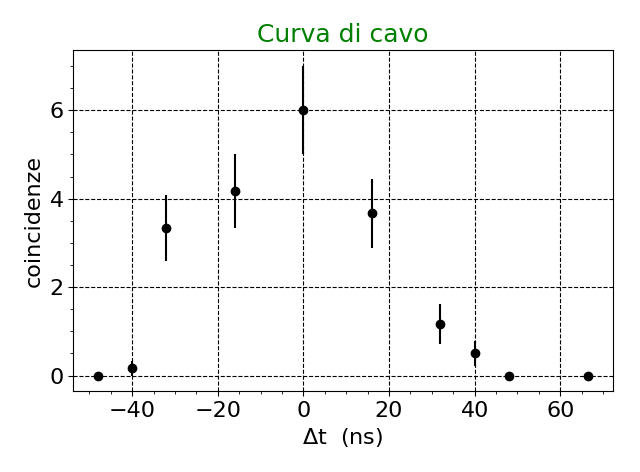
\includegraphics[width=8 cm]{curva_cavo}
\caption{Curva di cavo in funzione della differenza di tempi impostati sulle delay unit.}
\label{curv}
\end{figure}

% aggiungere il disegno di Giacomuzzo?
\end{section}


\begin{section}*{Rapporto segnale$/$fondo}

Dopo aver tolto le delay unit abbiamo variato la tensione di un PMT  e la soglia del discriminatore a cui era collegato mentre l'altro era lasciato ad un punto di lavoro costante in modo che non influenzasse le misure fatte sul primo. Abbiamo analizzato dapprima il PMT2 lasciando fisso il 4 ad una tensione nominale V$_4=1800$\! V ed una soglia V$_{thr_4}=-353\pm2$\! mV in modo che le concidenze casuali non potessero verificarsi in un intervallo di tempo di 10\! s. 
Il rapporto tra le coincidenze ed i conteggi rappresenta il rapporto tra segnale e segnale più rumore, in quanto il numero mostrato dallo scaler comprende sia i disturbi che le particelle. Il risultato è visibile in \emph{Figura \ref{test1}}.

\begin{figure}[h]
\centering
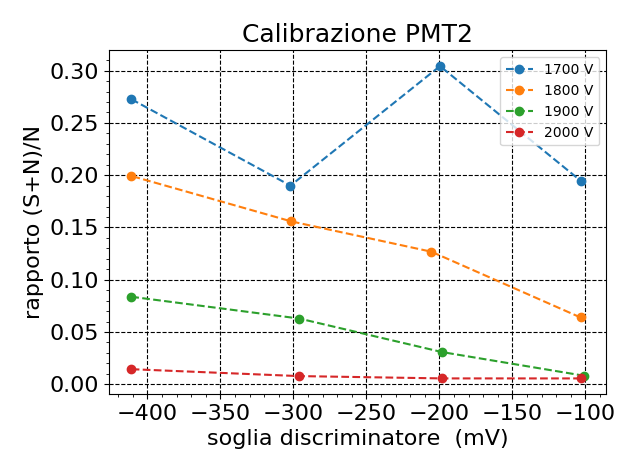
\includegraphics[width=8 cm]{calib_pmt2}
\caption{Rapporti S/(S+N) per il PMT2 in diversi punti di lavoro.}
\label{test1}
\end{figure}

La stessa cosa è stata fatta per il PMT4 lasciando il PMT2 al punto di lavoro V$_2=1820$\! V e V$_{thr_2}=-298\pm2$\! mV come mostrato in \emph{Figura \ref{test2}}.

\begin{figure}[h]
\centering
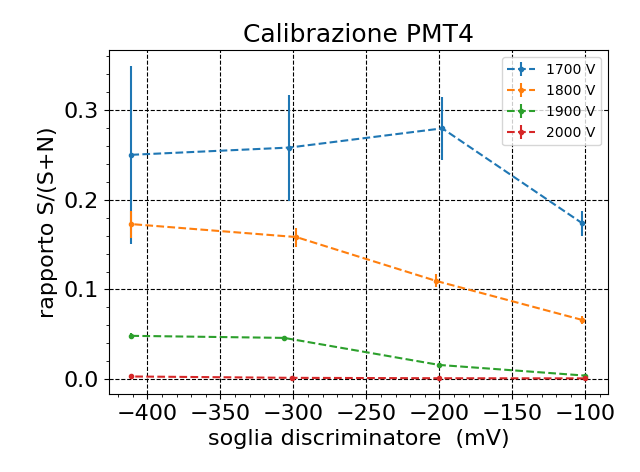
\includegraphics[width=8 cm]{calib_pmt4}
\caption{Rapporti S/(S+N) per il PMT4 in diversi punti di lavoro.}
\label{test2}
\end{figure}

\end{section}


\begin{section}*{Efficienza assoluta}

Per misurare l'efficienza assoluta del PMT3 è necessario eseguire i rapporti tra le coincidenze di tutti i tre rivelatori e quelle dei due più esterni. Per fare ciò abbiamo usato un secondo modulo di coincidenze per visualizzare quelle di tutti e tre. Non avendo ancora analizzato i dati riguardanti la sezione precedente, abbiamo stimato il punto di lavoro V$=1800$\! mV e V$_{thr}=-200$\! mV essere il migliore per i fotomoltiplicatori esterni. Quindi abbiamo variato soglia e alimentazione di quello centrale e disegnato il grafico di \emph{Figura \ref{eff}} per varie tensioni di alimentazione.

\begin{figure}[h]
\centering
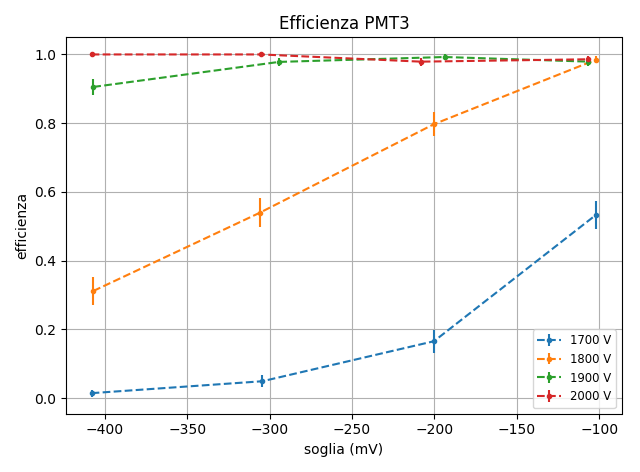
\includegraphics[width=8 cm]{efficienza}
\caption{Efficienza assoluta del PMT3.}
\label{eff}
\end{figure}

L'analisi effettuata contrassegna il punto di lavoro scelto prima come migliore perché il PMT che lavora in quelle condizioni ha una buona efficienza ed anche un buon rapporto S$/$(S$+$N). Quest'ultimo ci permette di avere meno coincidenze casuali ed evita la possibilità di overflow in caso di conteggi su un tempo molto lungo. L'efficienza corrispondente a questo punto di lavoro vale $\eta=80\pm3$\! \%. Possiamo adesso determinare il rate di particelle cosmiche avvalendoci della relazione 
$$ R_V=\frac{R_m}{1+R_m\Delta t} $$
in cui R$_m$è il rate misurato, R$_V$ quello vero e $\Delta t$ stimato in precedenza. Essendo quest'ultimo dell'ordine dei nanosecondi, R$_m\Delta t \ll 1$. Il rate misurato si ottiene dividendo le coincidenze a 3 per l'efficienza. Nel punto di lavoro in questione abbiamo osservato Quindi il rate di raggi cosmici risulta essere R$_V=14\pm1$\! particelle$/$s. Esso è inferiore alla metà di quanto atteso ma ciò è dovuto all'accettanza geometrica minore di uno.

\end{section}

\end{document}